\chapter{Systembeskrivelse} \label{ch:Systembeskrivelse}

Det system, der er tænkt realiseret i dette projekt, er en skalamodel af et drivhus med steppermotor til åbning af et vindue og blæsere til udluftning samt et varmelegeme til at varme drivhuset op. 
Til at måle på drivhuset var det tiltænkt at implementere en temperatursensor, jordfugtmålere samt sensorer til måling af lysintensitet og luftfugtighed. 
De to sidstnævnte er dog ikke implementeret grundet komplikationer i implementeringsfasen.

Selve systemet styres af et DevKit8000, som brugeren af systemet kan interagere med.
På denne platform kører - samtidigt med det grafiske miljø - processer til regulering og monitorering af miljøet i drivhuset.
Der er udover dette også mulighed for at tilgå forudindstillede planter i en plantedatabase samt at tilføje og fjerne eksisterende planter i et virtuelt drivhus, som systemet anvender til at afspejle de planter, der eksisterer i det fysiske drivhus.
Al aktivitet omkring styringen af systemet logges i en systemlog.

\begin{figure}[h]
\centering
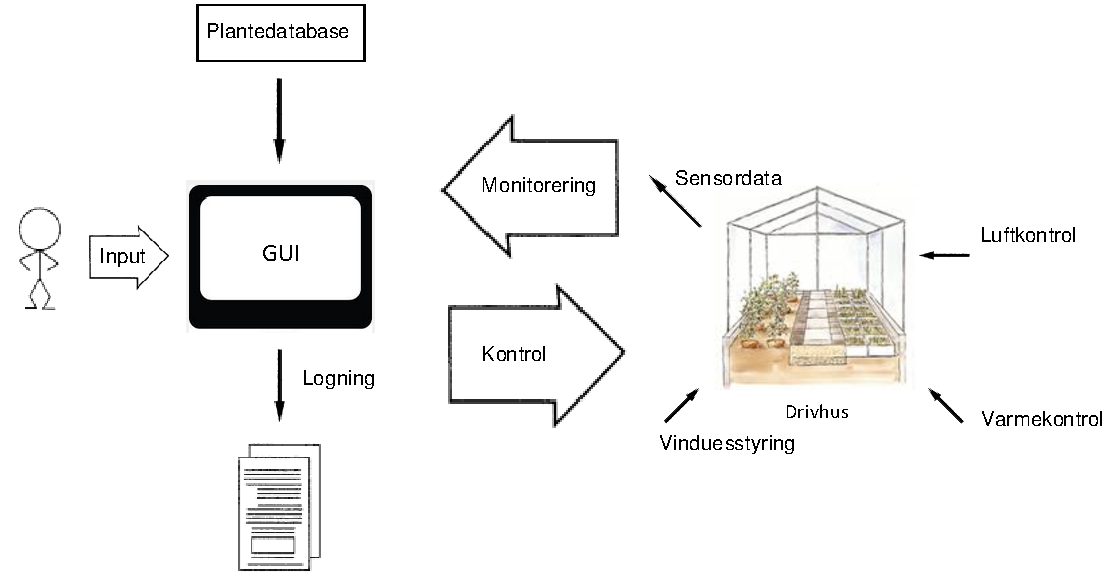
\includegraphics[width=\textwidth]{../fig/Rigt_Billede}
\caption{Rigt billede af systemet}
\label{fig:rigt_billede}
\end{figure}

Figur \ref{fig:rigt_billede} viser et rigt billede af systemet; der ses hvordan det fysiske drivhus påvirkes ved kontrol af varme og luft samt kommunikationen med GUI'en.

\clearpage

\begin{figure}[h!]
\centering
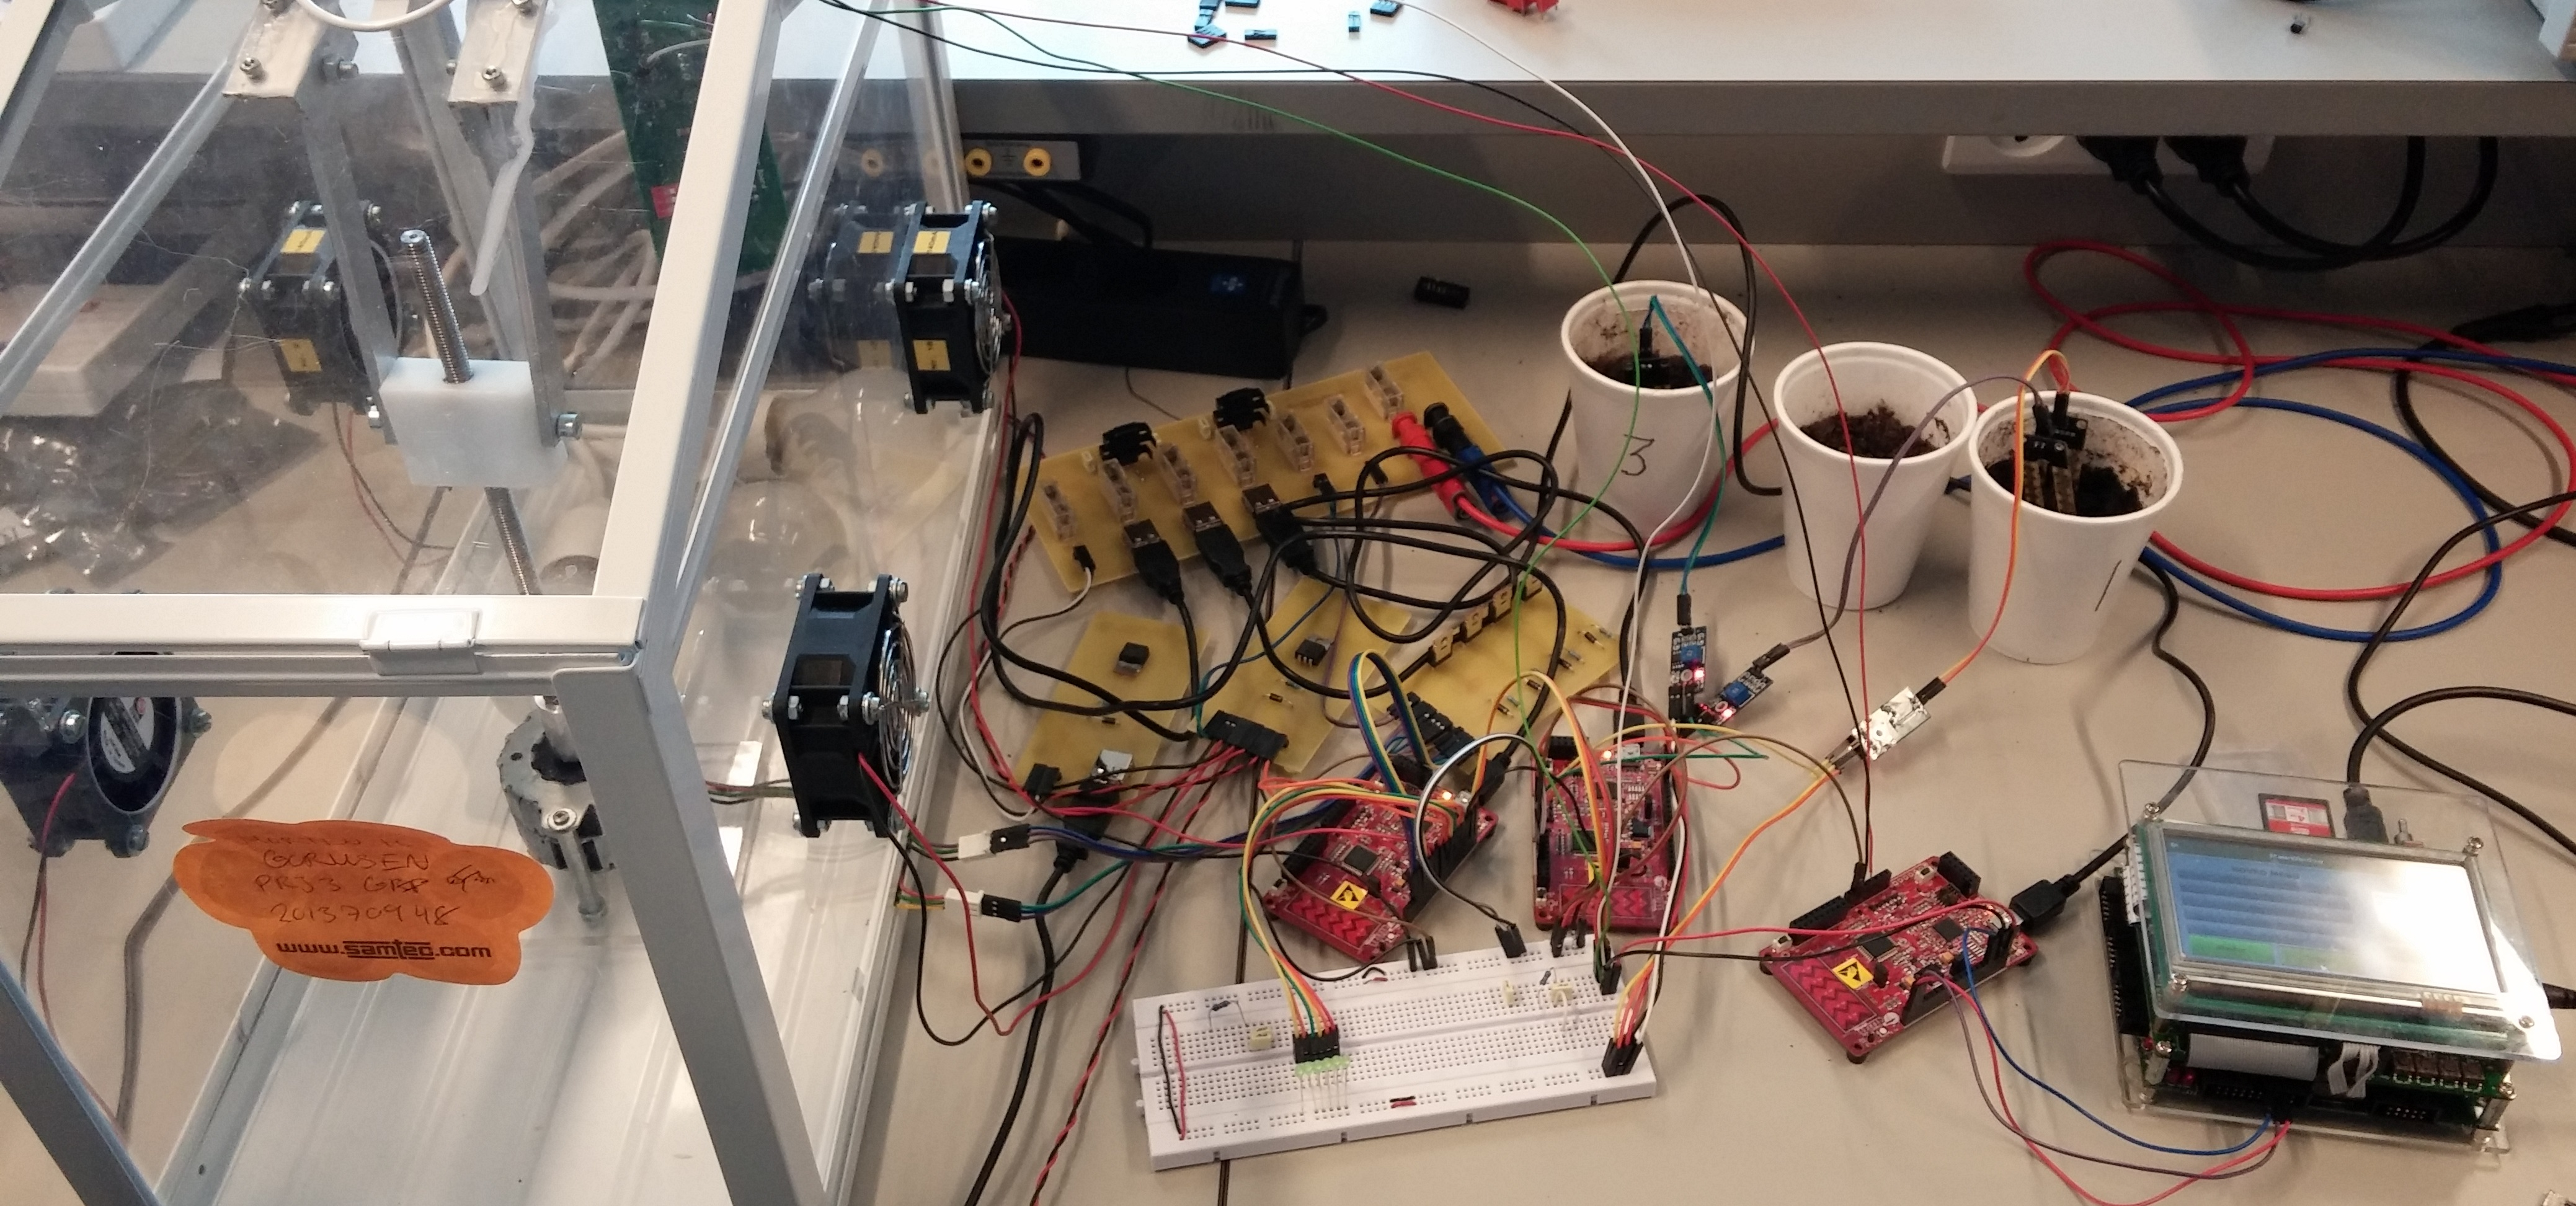
\includegraphics[width=\textwidth]{../fig/foto_system_crop}
\caption{Billede af det færdige system}
\label{fig:system_billede}
\end{figure}

På Figur \ref{fig:system_billede} ses et billede af den færdige prototype, og på Figur \ref{fig:gui_billede} ses et billede af hovedmenuen på systemets brugerflade.

\begin{figure}[h!]
\centering
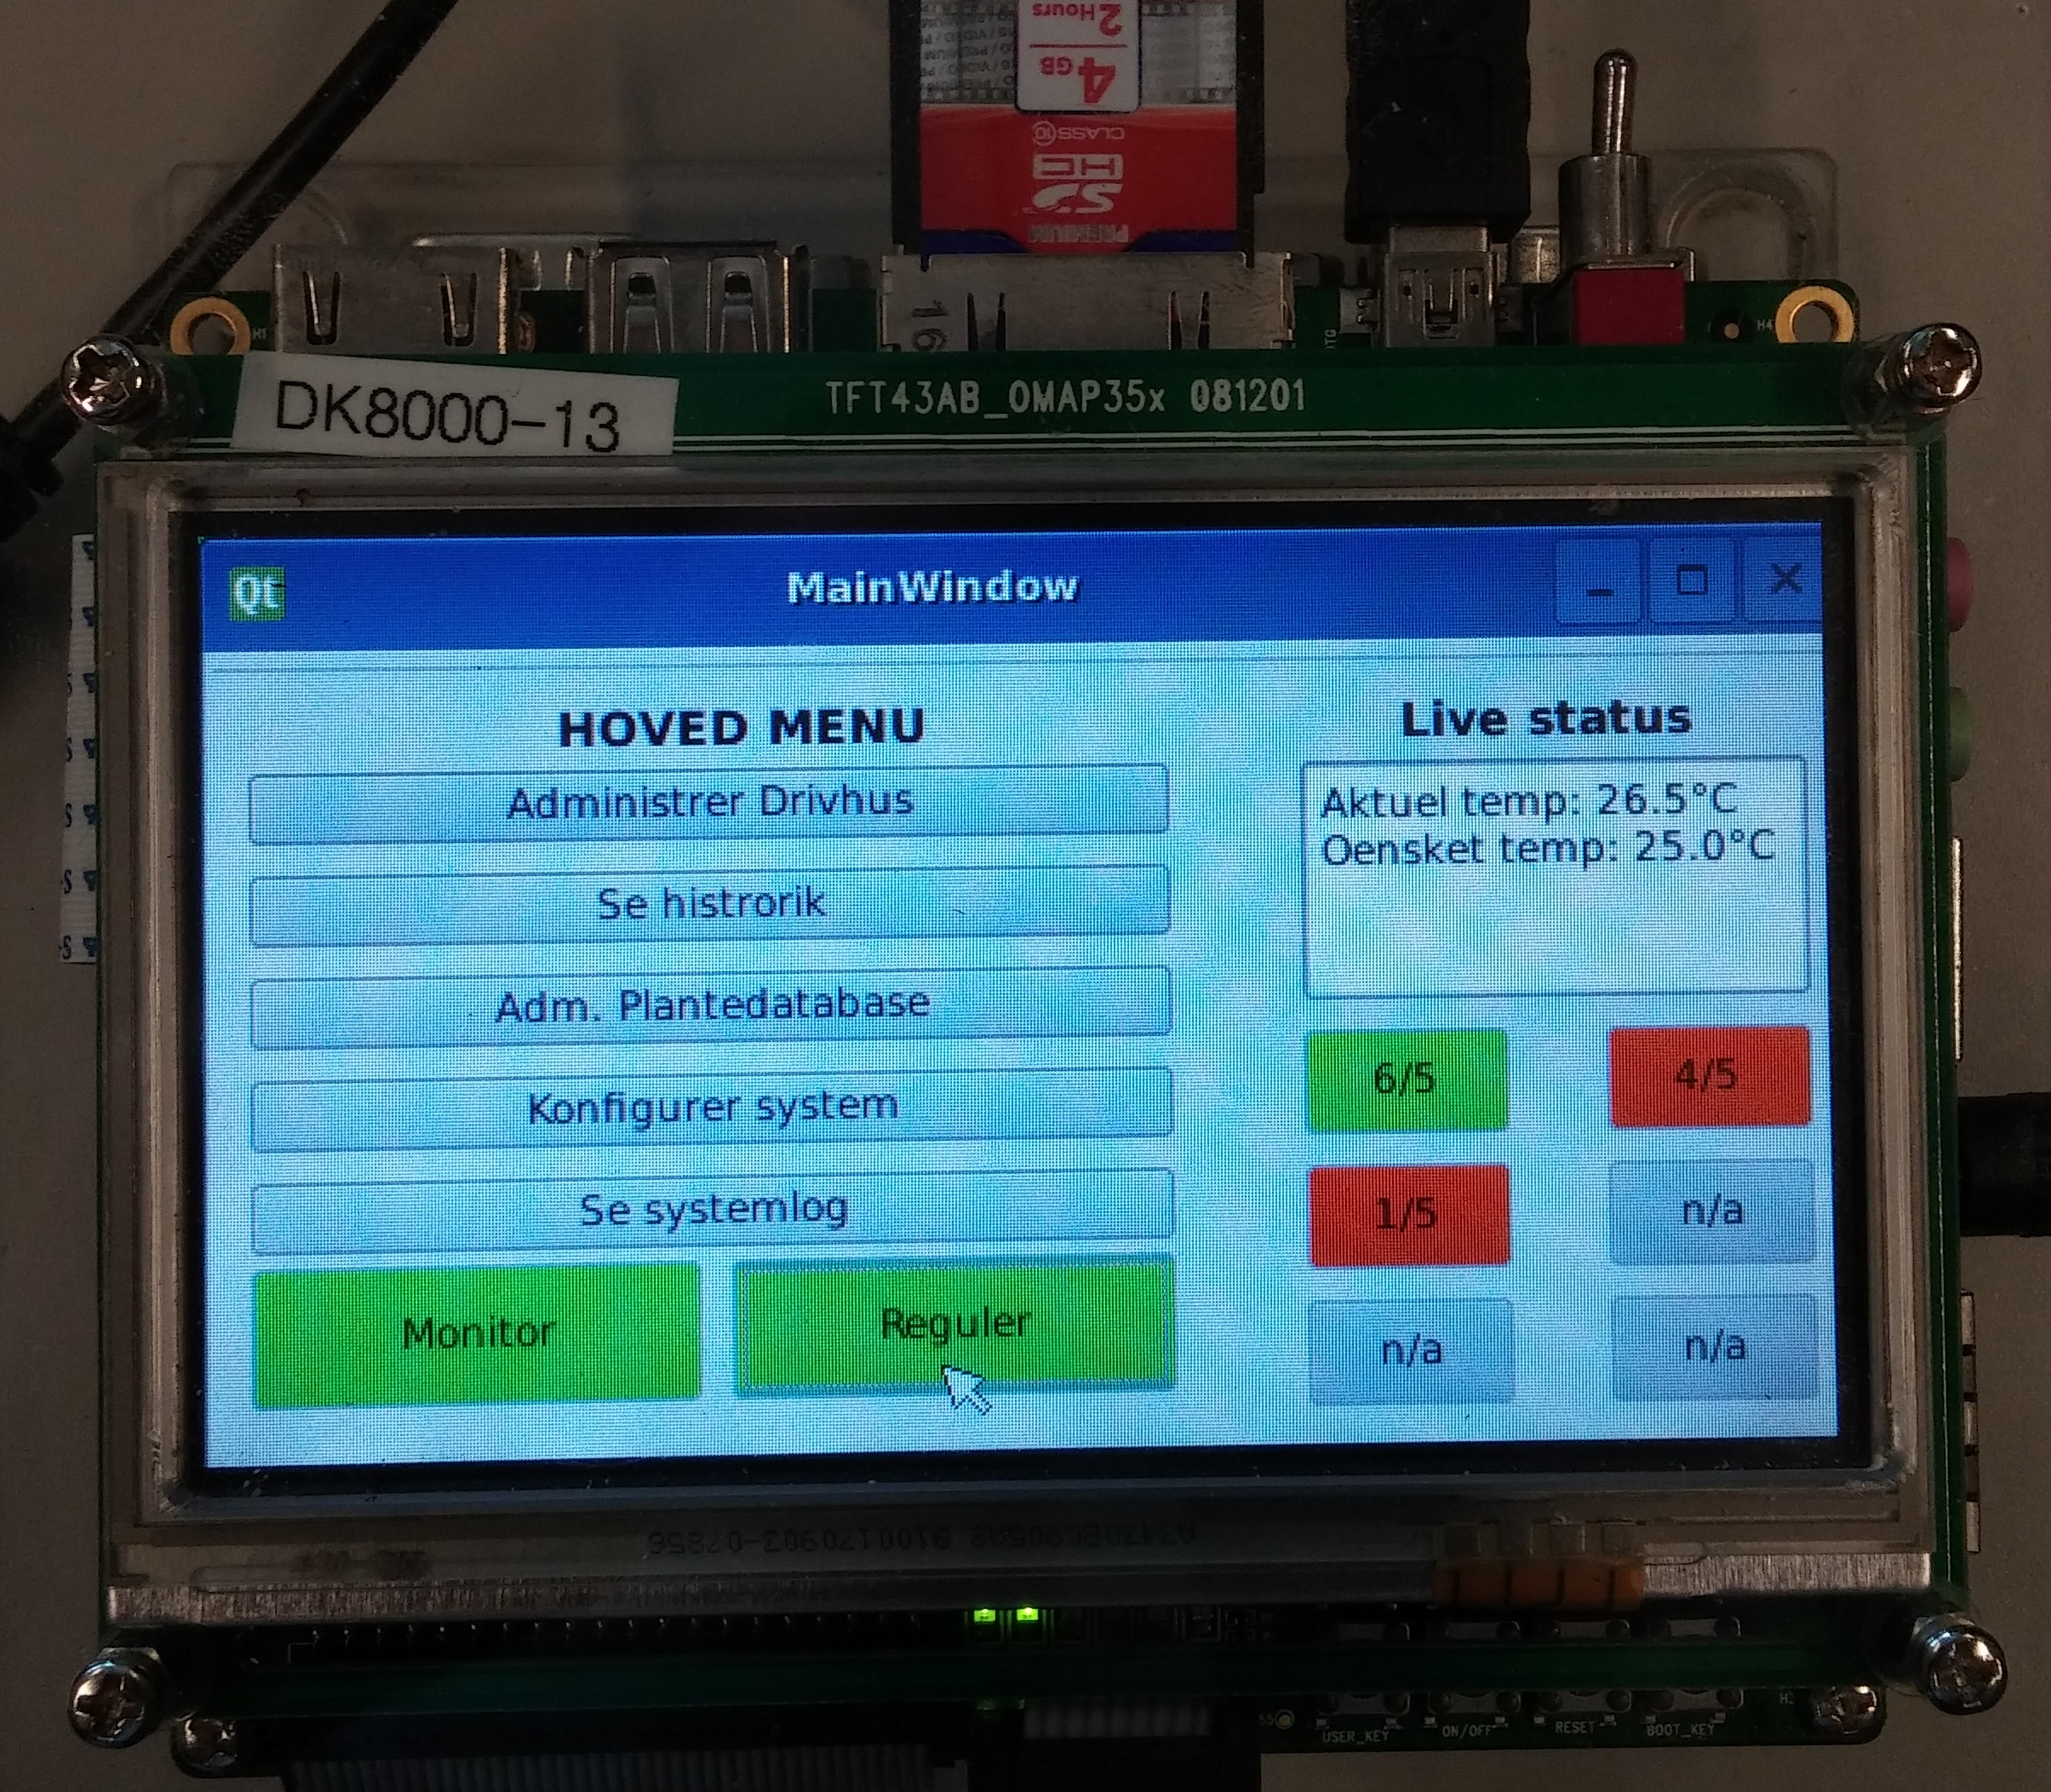
\includegraphics[width=\textwidth-5cm]{../fig/foto_gui_crop}
\caption{Billede af brugerfladen}
\label{fig:gui_billede}
\end{figure}